% !TeX encoding = UTF-8
% !TeX spellcheck = en_US
% !TeX root = presentation.tex
\subsection{KUKA youBot}
\begin{frame}{youBot Driver}
\begin{itemize}
	\item Driver for the KUKA youBot robot
	\item Includes youbot\_oodl node 
		\begin{itemize}
			\item Publishes to several topics and provides services for communication with the youBot
			\item Initializes the base and arm for communication
			\item Receives velocity commands for the base and arm, and position commands for the arm 
		
		\end{itemize}
	\item Uses ROS wrapper for translation to ROS
\end{itemize}

  
\end{frame}

%\begin{frame}
%\begin{itemize}
%	\item \textbf{ROS Wrapper}
%	\begin{itemize}
%		\item Allows to write ROS programs for controlling youBot
%		\item Provides an interface between youBot driver and ROS framework
%		\item Allows to move the base and arm by sending ROS messages
%	\end{itemize}
%	\item \textbf{List of Drivers}
%	\begin{itemize}
%		\item Drive base
%		\item Laser scanners
%		\item Arm 
%		\item Joystick
%		\item Transformations
%	\end{itemize}
%\end{itemize}
%\end{frame}
%-----------------------
\begin{frame}{Map building II}
\begin{itemize}
	\item \textbf{Problems}
		\begin{itemize}
			\item Messy Map
		\end{itemize}
	\item \textbf{Solutions}
		\begin{itemize}
			\item Incorrect transformation between laser frame and base link
		\end{itemize}
\end{itemize}
\end{frame}
%-----------------------
\begin{frame}{Map building II}
    \begin{center}
    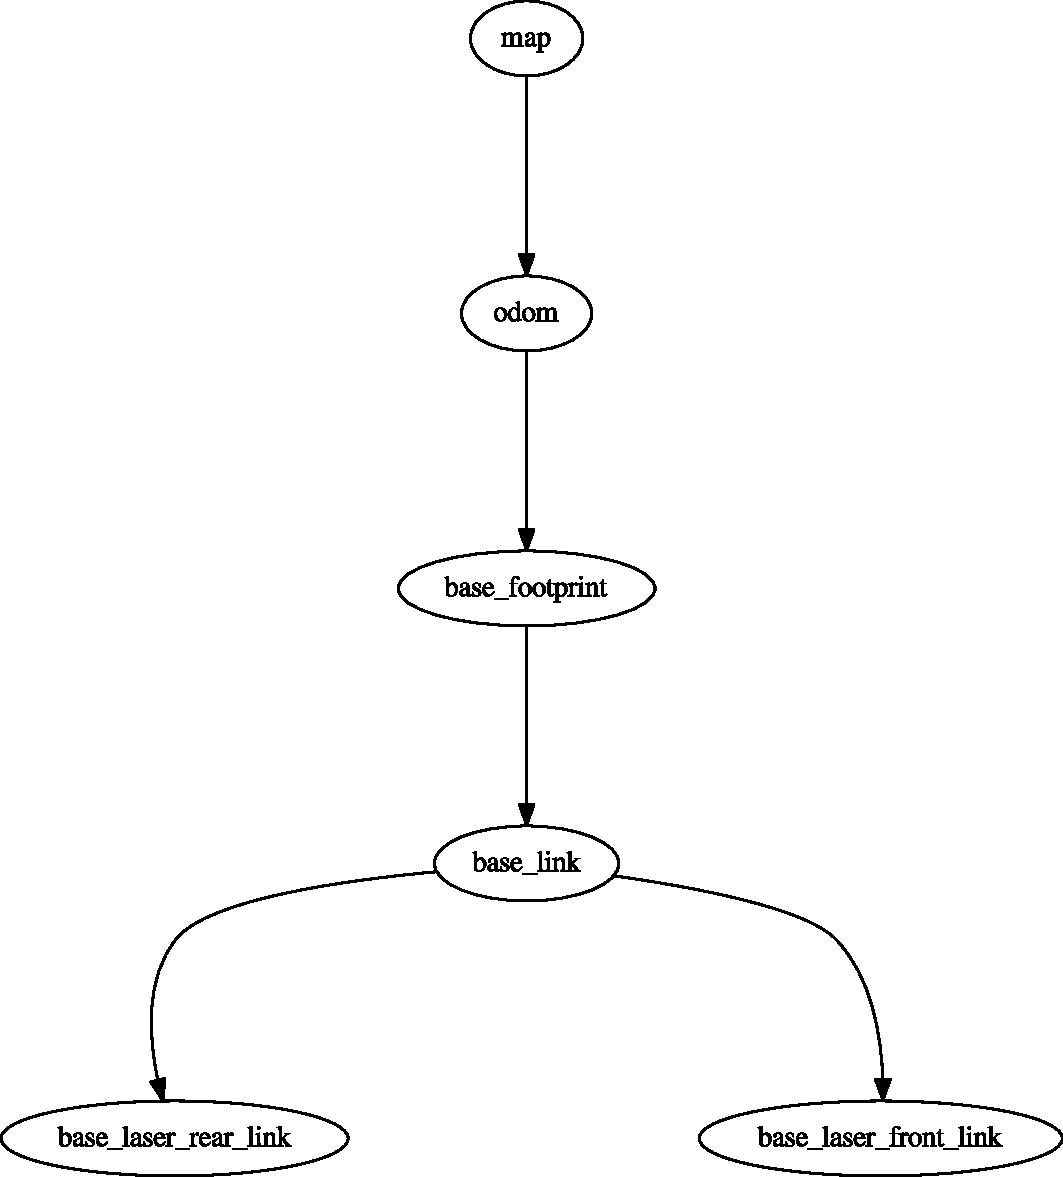
\includegraphics[width=0.6\textwidth]{gfx/frames_cleaned.pdf}
    \end{center}
\end{frame}
%-----------------------
\begin{frame}{Map building III}
    \centering
    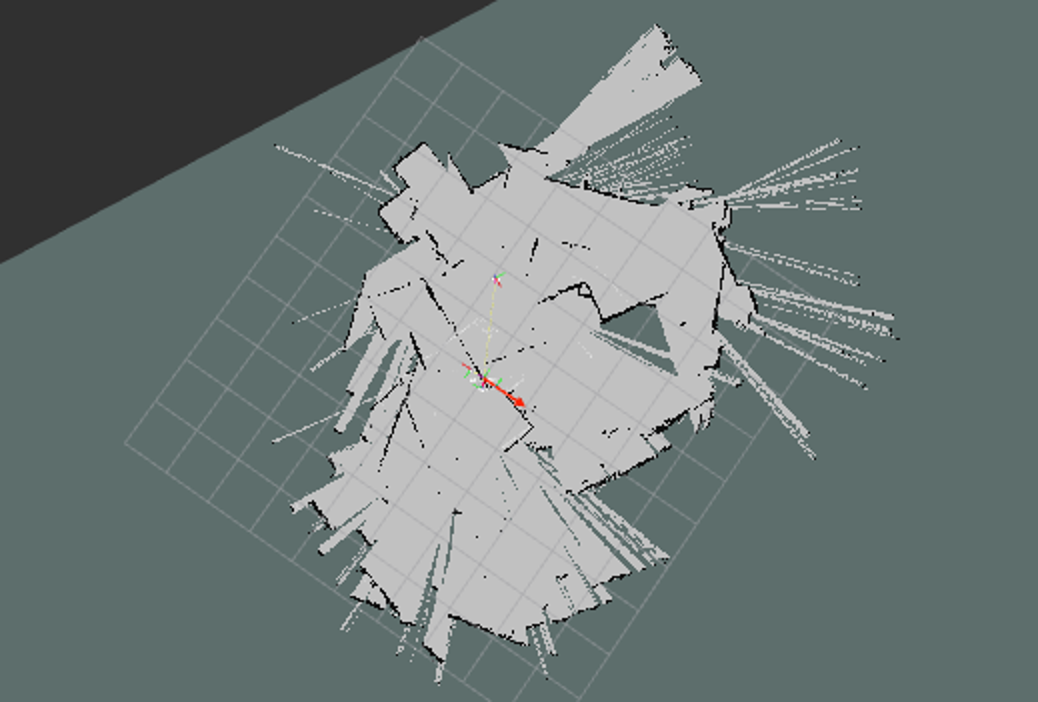
\includegraphics[width=0.9\textwidth]{gfx/map_messy.png}
\end{frame}
\begin{frame}{Map building IV}
\centering
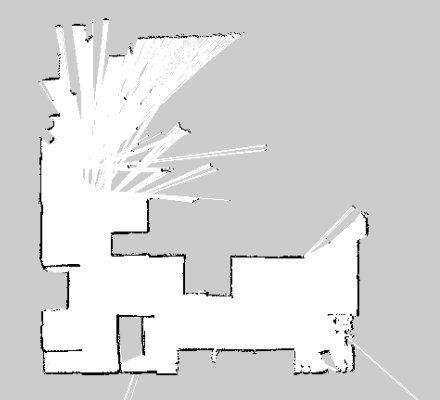
\includegraphics[width=0.8\textwidth]{gfx/map.png}
\end{frame}

%-----------------------
\begin{frame}{Localization II}
\begin{itemize}
\item \textbf{Problems}
    \begin{itemize}
    \item Amcl is not working
    \item Amcl cannot localize robot when it is in the end of arena
    \end{itemize}
\item \textbf{Solutions}
	\begin{itemize}
	\item Parameter odom\_model\_type should be omni\-corrected
	\item Arena was changed a lot, so sensor reading cannot be related to map
	\end{itemize}
\end{itemize}
\end{frame}
%-----------------------
\begin{frame}{Navigation}
\begin{itemize}
	\item Requirements
		\begin{itemize}
			\item Map (map\_server)
			\item Localization (amcl)
			\item Odometry source
			\item Transforms
			\item Sensor sources
			\item Goal (move\_base) 
		\end{itemize}
	\item Planners: global, local
	\item Costmaps: global, local
	\item Local planner: dwa\_local\_planner
		\begin{itemize}
			\item Given: plan, costmap, odom
			\item Generates costs of transversing through map grids
			\item Output: Velocity command
		\end{itemize} 
	\item Output: Velocity command (cmd\_vel)
\end{itemize}
\end{frame}
%-----------------------
\begin{frame}{Path executor}
    
    Path executor reads  a set of user inputs and convert them to move\_base\_msgs.
    \begin{itemize}
        \item Class: Position, Pose, Environment, Workspace, PathExecutor
        
        \item Functions:
        \begin{itemize}
        	\item Reads user inputs
        	\item Reads workspace from file
            \item Converts workspace to move\_base\_msgs
            \item Clears cost map
            \item Sends goal message
        \end{itemize}
    \end{itemize}
    
\end{frame}
